% The text in this file should contain an overview of the new MDAO environment/process we are developing as well as OpenMDAO

As stated in the Introduction, the UAM concept development to date has focused on identifying a set of vehicle designs and the discipline areas where further refinement is needed to improve the designs.
Given the multidisciplinary design challenges presented by these new UAM vehicle concepts, the objective of this research is to develop a multidisciplinary analysis and optimization environment capable of addressing these needs.
This analysis environment therefore needs to contain separate analysis tools for each of the disciplines under consideration.
Furthermore, these disciplinary tools needs to be tightly integrated to enable the optimization of the overall vehicle system.
The large potential size of the design space for these vehicles also leads to the use of gradient based optimization techniques in this process.
Applying gradient based optimization algorithms requires determining total derivatives of the system and its components.
To support this requirement, the analytic computation of derivatives was determined to be an important feature as it provides highly accurate derivatives with reduced computational cost.
Overall, these requirements for the multidisciplinary analysis environment guided the development of this system as described in this section.

With these requirements for the multidisciplinary design and analysis environment, a number of tools were developed then integrated together to form the overall optimization capability.
% This development is summarized in Figure \ref{f:stack}.
The disciplinary tools were created to provide a physics-based analysis capability at the conceptual design level.
In addition, the tools were also developed with analytic derivatives built in to better enable gradient based optimization.
Each of these tools were then tightly integrated together in an overall analysis framework to conduct the optimization.
The first section below describes this optimization framework and is followed by brief descriptions of each of the disciplinary tools at the library and analysis levels developed in support of this research. 
The full aircraft model developed will be the focus of the optimization study described in Sections \ref{sec:opt_prob} and \ref{sec:opt_results}.


% \subsection*{Integration and Optimization Framework}

% Paragraph largely copied from Aviation 2017 paper, need to rewrite
The OpenMDAO framework was used in this study to develop, integrate and optimize the disciplinary analysis tools for the study of UAM vehicles.
OpenMDAO is an open source analysis framework being developed by NASA which is written in the Python programming language.\cite{gray_openmdao2010_b,gray2014automatic,openmdao}
It is designed to enable the multidisciplinary design, analysis and optimization of complex systems.
In this capacity, it provides the ability to couple different disciplinary analysis tools, often written in different programming languages, into a single analysis or optimization process.
In addition, the OpenMDAO framework provides access to a number of nonlinear solvers, design of experiments drivers, gradient based optimizers and gradient free optimizers.







% Given these challenges, a new tool set and tightly coupled multidisciplinary design process is being developed
% Goal is to provide enhanced modeling capabilities across the disciplines as well as improvements to enable gradient based optimization
% Existing tools were generally deemed inadequate as they do not provided analytic derivatives
% Therefore, new tools (often implementing the same physics) were created
% These tools and the models used to analyze the tiltwing vehicle will be described in later sections


% Existing process used by RVLT used a loose coupling between disciplines to develop designs
% New process formulated in this research aimed to more tightly integrate disciplines
% Top-level description of the new design method is shown in the following figures
% As shown in the first figure, the design optimization process is generally comprised of two major elements
% The first is a set of discipline design models which size the aircraft components for a given set of performance requirements
% Information about the design of these components is then passed to the second major element which evaluates and the mission performance
% An optimizer is applied around these two elements to vary the discipline design variables and optimal control variables to minimize the objective subject to a number of constraints
% The next two figures detail the modeling environments created in each of these two major elements
% The first provides the disciplinary design model setup
% This major element contains components which completed the design sizing of the electrical and turboshaft elements of the propulsion system as well as computing the mass of the various aircraft components
% The second figure shows the mission performance major element
% As shown in this figure, the three propulsion system components are evaluated to determine the required fuel flow given the thrust control
% Furthermore, the wing aerodynamic and structural performance is evaluated to support calculation of the flight dynamics and the state rates
% All of this data is generated at a number of points throughout the mission profile which is then used to determine the optimal control settings for the aircraft/flight




\begin{figure}[htb]
\begin{center}
 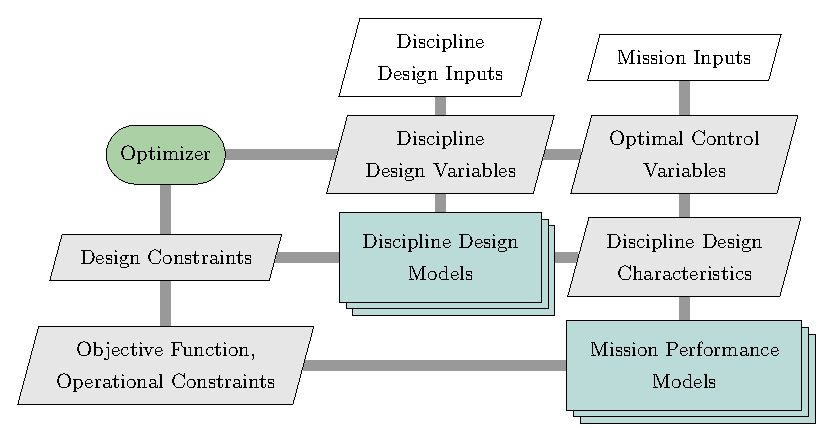
\includegraphics[scale=1.0]{../Images/General_XDSM.pdf}
 \caption{Multidisciplinary Analysis Environment.}
 \label{f:framework}
\end{center}
\end{figure}

\begin{figure}
\begin{center}
 % \textbf{!!!!! Create XDSM of Design/Static Calculations !!!!!}
 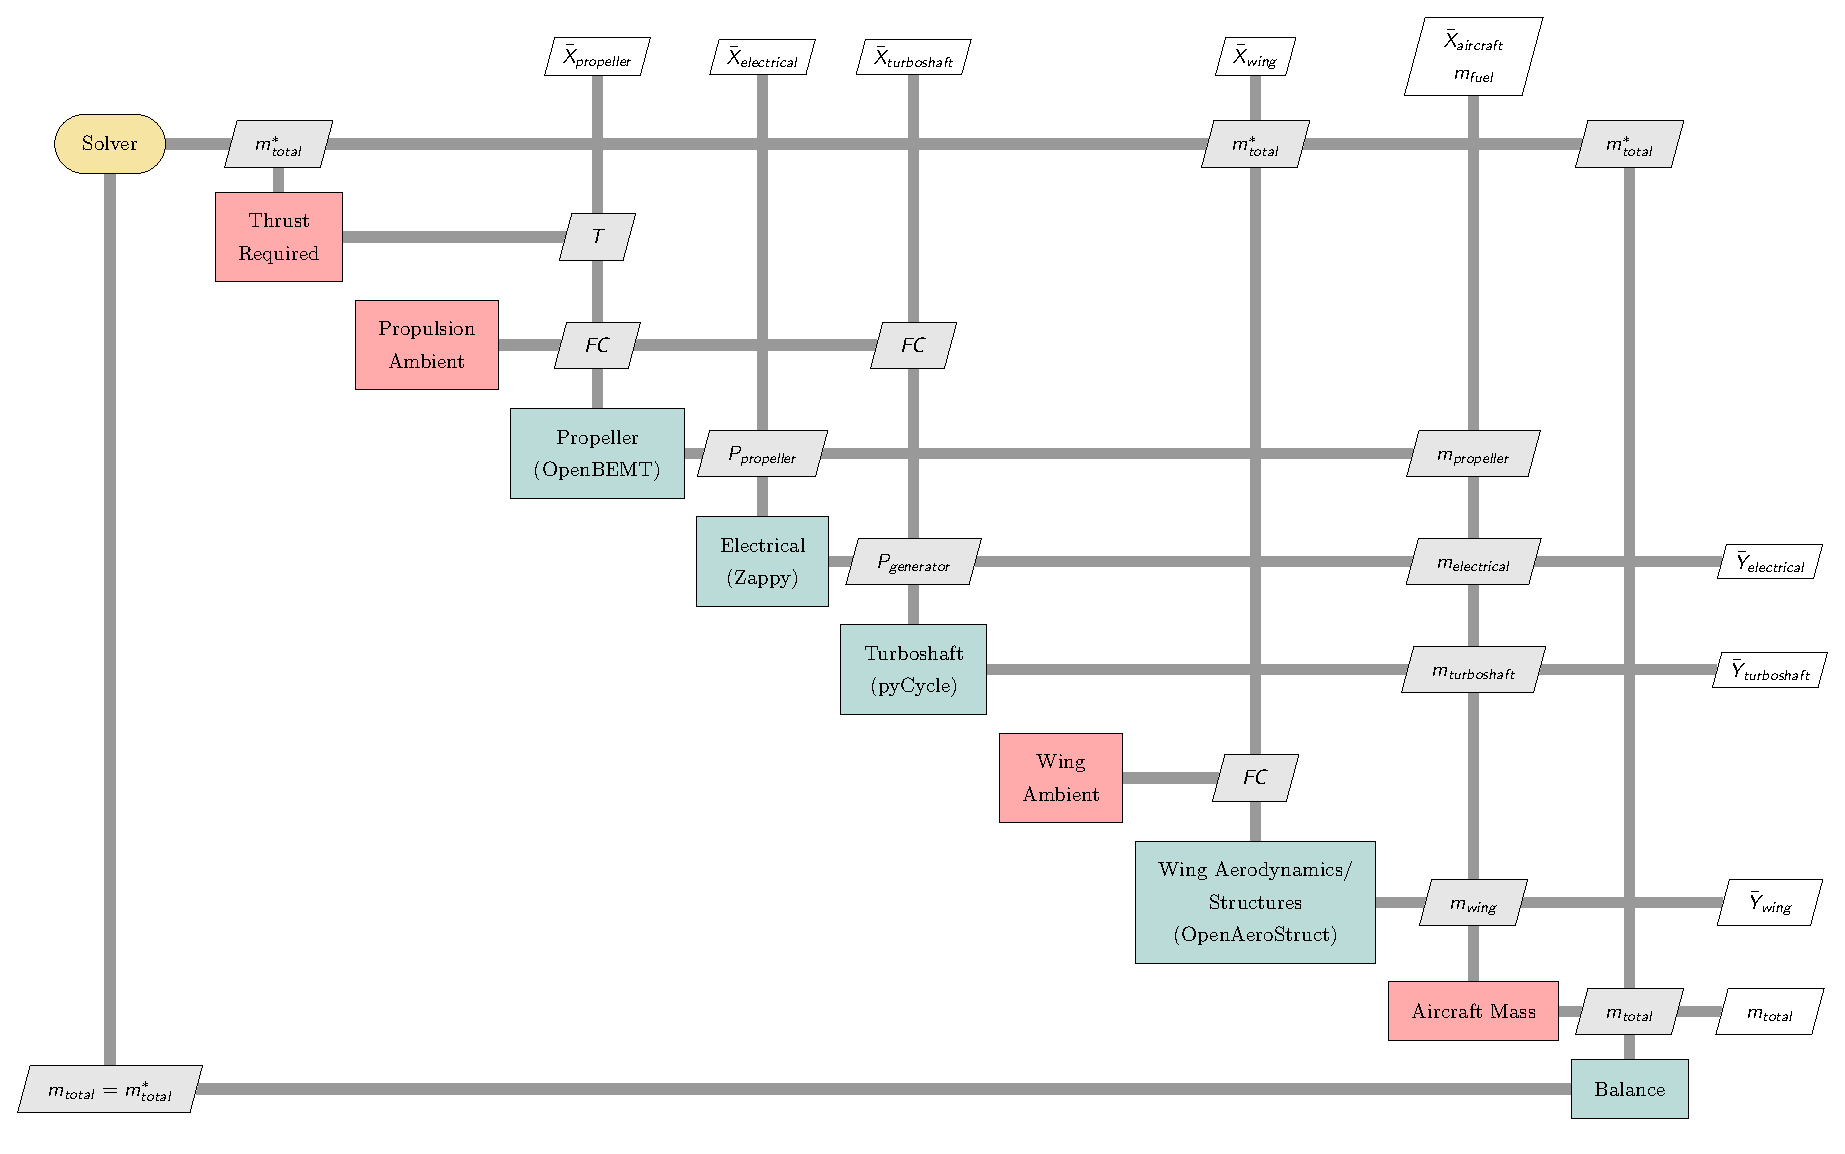
\includegraphics[width=1.0\textwidth]{../Images/Design_XDSM.pdf}
 \caption{Discipline Design Modeling.}
 \label{f:design}
\end{center}
\end{figure}

\begin{figure}
\begin{center}
 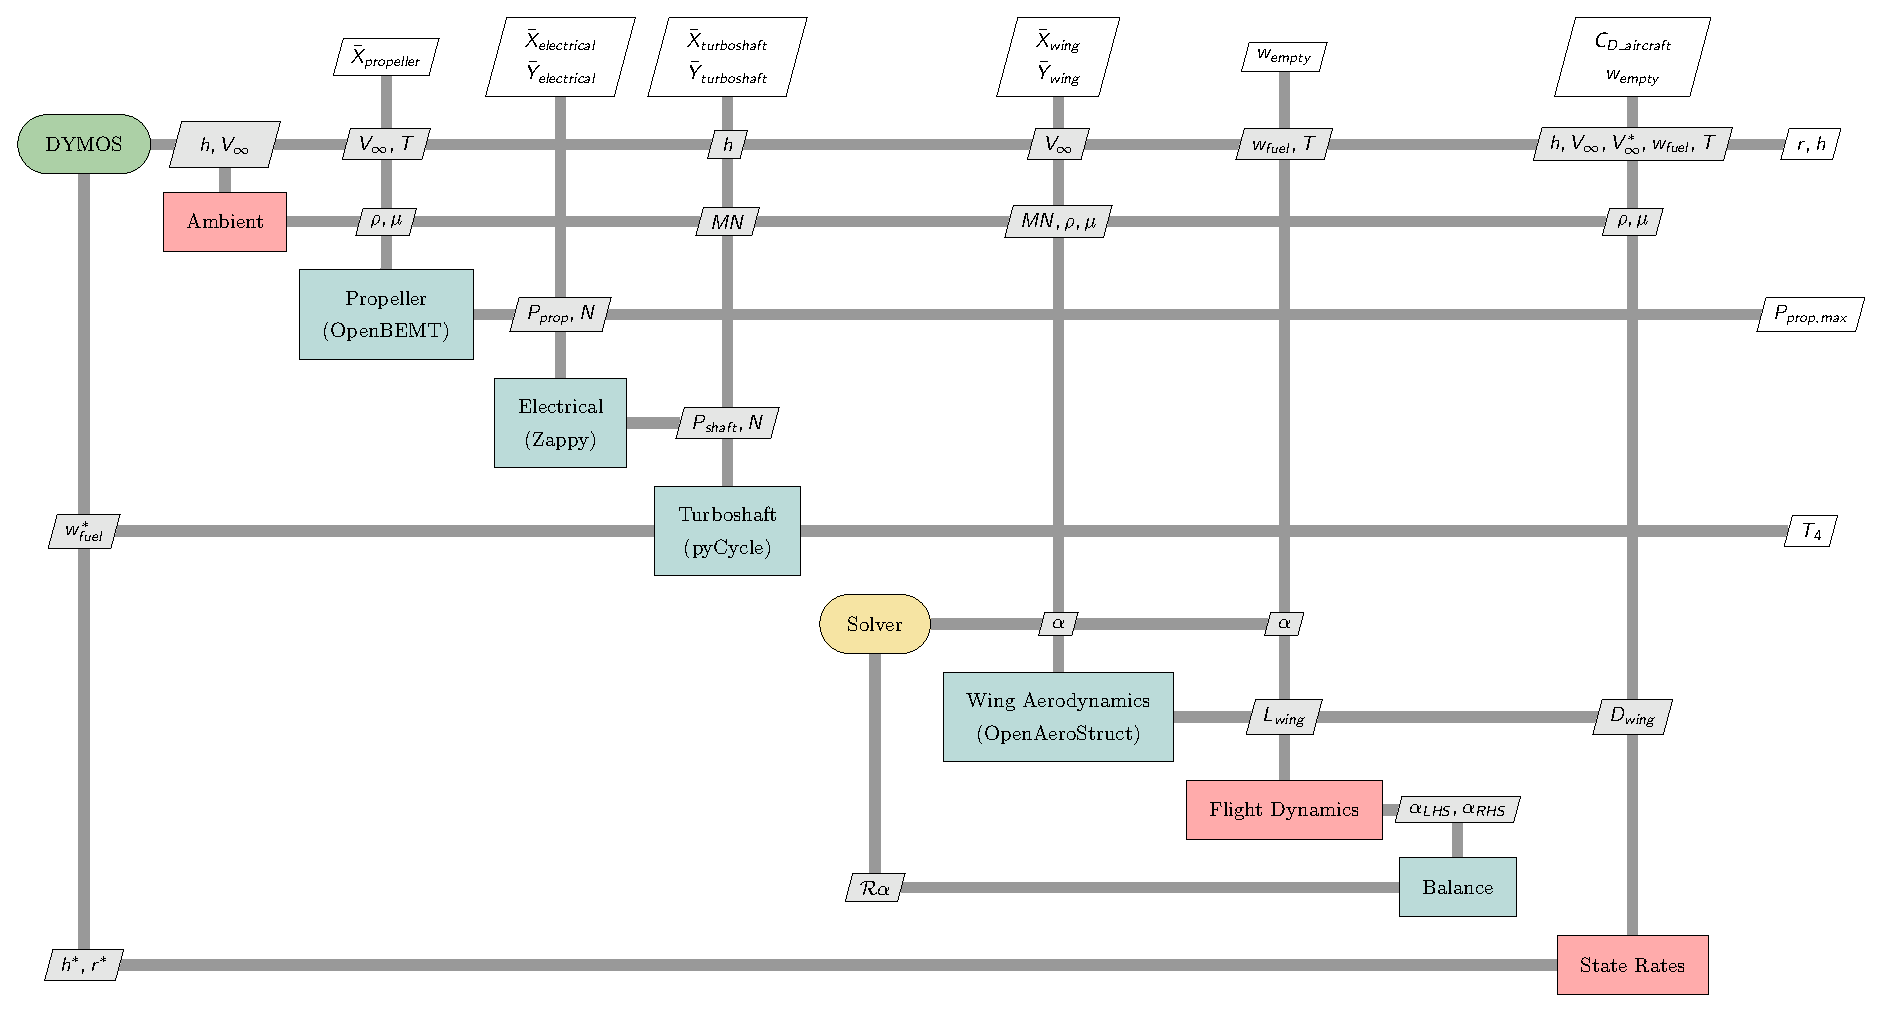
\includegraphics[width=1.0\textwidth]{../Images/Mission_XDSM.pdf}
 \caption{Mission Performance Modeling.}
 \label{f:mission}
\end{center}
\end{figure}


As can be seen in Figures \ref{f:design} and \ref{f:mission}, there are four primary disciplines included in the MDAO environment being developed in this work.  
These disciplines include propulsion, wind aerodynamics and structures, aircraft mass, and optimal control and trajectory analysis.
The next sections will describe the individual disciplinary tools created to support the above multidisciplinary design process as well as the specific models developed to represent the tiltwing vehicle under consideration in this paper.



% \begin{figure}
% \begin{center}
%  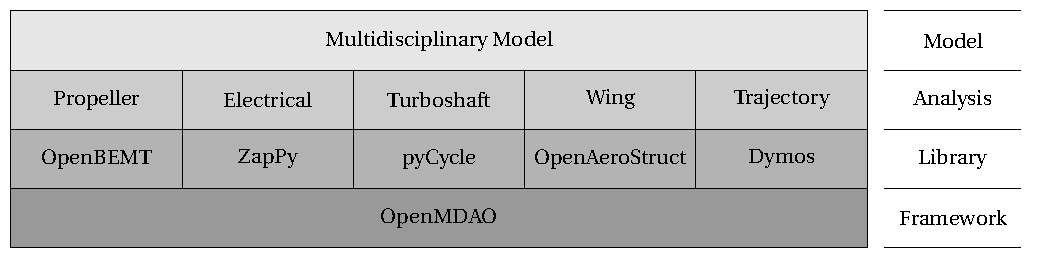
\includegraphics[width=\textwidth]{../Images/software_stack.pdf}
%  \caption{Multidisciplinary Analysis tool Softwary Stack.}
%  \label{f:stack}
% \end{center}
% \end{figure}


For each disciplinary analysis, include the foollowing information:
\begin{itemize}
    \item Describe the analysis tool and summarize the physics captured by the tool
    \item Describe the inputs and outputs of the code
    \item Make sure to include both design/static information as well as ODE information as appropriate
    \item Reference previous publications on the tool
    \item Describe the model created using the tool for the tiltwing UAM vehicle (include graphic as needed)
\end{itemize}

